\documentclass[a4paper, 11pt]{article}
\usepackage[utf8]{inputenc}
\usepackage[a4paper,top=0.5cm,bottom=1cm,left=1cm,right=1cm,marginparwidth=1.5cm]{geometry}
\usepackage{graphicx}

\title{Climate Change in Florida}
\author{PU ZHAO}
\date{}
\begin{document}
\maketitle

\section{Introduction}

The project is divided into three steps. First, the correlation coefficient between the year and temperature in Key West, Florida, during the 20th century was calculated. Second, the temperature was randomly assigned to the year and the correlation coefficient was calculated and stored multiple times. Finally, It is to calculate the proportion of correlation coefficients of all randomly assigned samples that are greater than the initial correlation coefficient.

\section{Results and Interpret}
\subsection{}
Correlation Coefficient of the original year and temperature of Florida= 0.5331784 

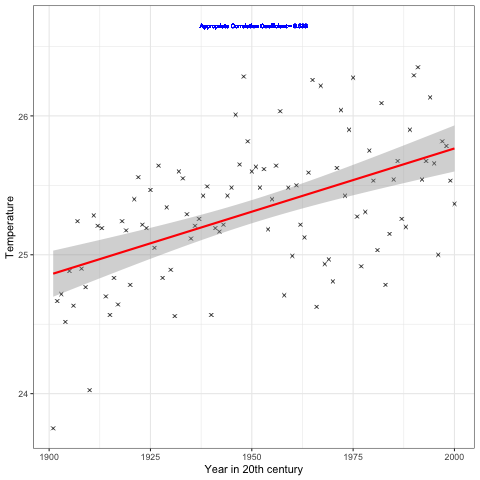
\includegraphics[scale=0.35]{../data/ats_plot.png}

\subsection{}
The figure below is the density of correlation coefficients of 10,000 random temperatures to years in Florida. The temperature in Florida is randomly assigned to the year and repeated 10,000 times. The correlation coefficient is calculated and stored. The line in the figure is the original correlation coefficient of Florida.

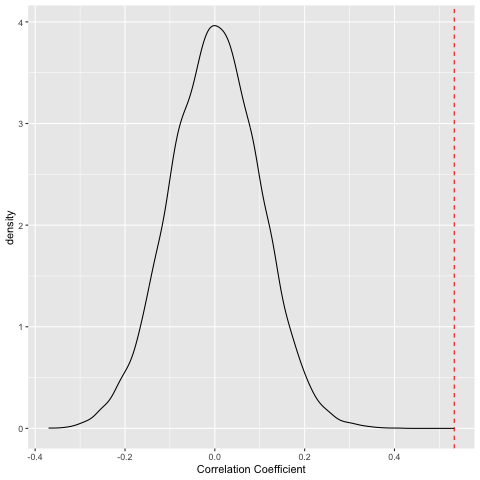
\includegraphics[scale=0.35]{../data/random_ats_plot.png}

\subsection{}
The fraction of the random correlation coefficients were greater than the observed one is 0. It can also be seen from the above density figure.
\end{document}



